\documentclass[11pt]{article}
\usepackage[margin=0.9in]{geometry}
\usepackage{amsmath,amssymb,booktabs,graphicx}
\pagestyle{empty}
\begin{document}
\section*{Harmonic fit of Migkas $A(\ell)$ set equal to the Sedov--Taylor + Gauss tidal model}

\paragraph{Notation.} $r$: radius of our vision shell (horizon), centred on us, $r\simeq14.3$ Gpc $\simeq46.5$ Gly comoving.
$D$: our distance from the CoE, beyond the horizon, so $d<r<D$. $d$: source (cluster) depth from us. $R$: distance from the CoE; $R_S$ for a source.
$L$: density scale length. $\kappa\equiv GM(<D)/(H_0^2D^3)=M(<D)/[2M_{\rm crit}(<D)]$ (definition used in the numerical model; uniform $\Omega_m$ gives $\kappa=\Omega_m/2$).

\paragraph{Model.} Let $\vec D$ point from the CoE to us, so $\hat D$ is the anti-CoE axis $(\ell_0,b_0)$, and let $\mu=\hat n\cdot\hat D=\cos\theta$ for line of sight $\hat n$.
A source at $\vec R_S=\vec D+d\,\hat n$ has (law of cosines) $R_S^2=D^2+d^2+2Dd\,\mu$. For a point-mass ($1/R^2$) field the peculiar velocity is $\vec u=-k\vec R/R^3$, and
$\delta H=(\vec u_S-\vec u_O)\cdot\hat n/d=(k/D^3)\left[(3\mu^2-1)+\tfrac{d}{D}\left(\tfrac92\mu-\tfrac{15}{2}\mu^3\right)+O(d^2/D^2)\right]$
(checked numerically: next-order coefficients $4.5000,\,-7.5000$; for $d/D<0.022$ the neglected terms are $\sim5\times10^{-4}$ of the leading term), hence
\begin{equation}
\frac{A}{A_{\rm all}} = N\left[1+\alpha\kappa\,(3\mu^2-1)+\alpha\kappa\,\frac{d}{D}\left(\tfrac92\mu-\tfrac{15}{2}\mu^3\right)\right].
\end{equation}
In the Galactic plane, $\mu=c\cos x$ with $c\equiv\cos b_0$, $x\equiv\ell-\ell_0$. Using
$\cos^2x=\tfrac12(1+\cos2x)$ and $\cos^3x=\tfrac14(3\cos x+\cos3x)$, and the $90^\circ$ sector window
$W_m=\dfrac{\sin(m\pi/4)}{m\pi/4}$ ($W_1=0.900,\ W_2=0.637,\ W_3=0.300$):
\begin{align}
\frac{A}{A_{\rm all}} ={}& N\left[1+\alpha\kappa\left(\tfrac32c^2-1\right)\right]
+ N\alpha\kappa\,\frac{d}{D}\,c\left(\tfrac92-\tfrac{45}{8}c^2\right)W_1\cos x \nonumber\\
&+ N\alpha\kappa\,\tfrac32c^2\,W_2\cos2x
- N\alpha\kappa\,\frac{d}{D}\,\tfrac{15}{8}c^3\,W_3\cos3x .
\end{align}

\paragraph{Data.} Linear least squares to the 71 digitized points of Migkas et al.\ (2020), Fig.~6:
\begin{equation}
\frac{A}{A_{\rm all}} = 0.9965 + 0.0296\cos\ell + 0.0434\sin\ell + 0.0636\cos2\ell + 0.0366\sin2\ell - 0.0299\cos3\ell - 0.0114\sin3\ell,
\end{equation}
$R^2=0.915$ (dipole+quadrupole only: $R^2=0.814$). Quadrupole phase: $\ell_2=15.0^\circ$.

\paragraph{Term-by-term equality} (data coefficient of $\cos m(\ell-15^\circ)$):
\begin{align}
m=0:&\quad 0.9965 = N\left[1+\alpha\kappa\left(\tfrac32c^2-1\right)\right]\\
m=1:&\quad +0.0398 = N\alpha\kappa\,\frac{d}{D}\,c\left(\tfrac92-\tfrac{45}{8}c^2\right)W_1\\
m=2:&\quad +0.0733 = N\alpha\kappa\,\tfrac32c^2\,W_2\\
m=3:&\quad -0.0292 = -N\alpha\kappa\,\frac{d}{D}\,\tfrac{15}{8}c^3\,W_3
\end{align}

\paragraph{Manipulations.}
\begin{align}
\frac{m=1}{m=3}:&\quad \frac{\left(\tfrac92-\tfrac{45}{8}c^2\right)W_1}{-\tfrac{15}{8}c^2W_3}=\frac{0.0398}{-0.0292}
\;\Rightarrow\; c^2=0.695,\ |b_0|=33.5^\circ\\
\frac{m=3}{m=2}:&\quad \frac{0.0292}{0.0733}=\tfrac54\,c\,\frac{W_3}{W_2}\,\frac{d}{D}
\;\Rightarrow\; \frac{d}{D}=0.81\\
m=2:&\quad N\alpha\kappa=\frac{0.0733}{\tfrac32c^2W_2}=0.1105\\
m=0:&\quad N=0.9918,\qquad \alpha\kappa=0.111
\end{align}

\paragraph{Formal solution.} $\ell_0=15.0^\circ$, $|b_0|=33.5^\circ$, fitted ``$d/D$''$\,=0.81$, $\alpha\kappa=0.111$, $N=0.992$;
all four equations are satisfied exactly; $R^2=0.780$ against the 71 points.
The components perpendicular to the axis (coefficients of $\sin m(\ell-15^\circ)$: $+0.0342,\,-0.0001,\,+0.0131$)
cannot be produced by any axisymmetric model; the dipole direction $\ell_1=56^\circ$ is $41^\circ$ off axis.

\paragraph{Physical interpretation for $d<r<D$.}
Median Migkas redshift $z=0.075$ (Migkas et al.\ 2020, Sect.~2), $H_0=70\ \mathrm{km\,s^{-1}\,Mpc^{-1}}$:
\begin{align}
d &\simeq \frac{cz}{H_0}=\frac{(2.998\times10^5)(0.075)}{70}\ \mathrm{Mpc}= 321\ \mathrm{Mpc}\approx 1.05\ \mathrm{Gly},\qquad
r\simeq14.3\ \mathrm{Gpc}\approx46.5\ \mathrm{Gly},\\
D&>r\ \Rightarrow\ \frac{d}{D}<\frac{d}{r}=\frac{0.321}{14.3}=0.022\qquad(\text{and } d/D<r/D<1\ \text{for any source inside the shell}).
\end{align}
Putting $d/D=0.022$ into Eqs.~(5) and (7), with $N\alpha\kappa$ from Eq.~(6), for $|b_0|=33.5^\circ,\ 0^\circ,\ 15^\circ$:
\begin{align}
m=3:&\quad -N\alpha\kappa\,\tfrac{d}{D}\,\tfrac{15}{8}c^3W_3=-0.00081,\ -0.00097,\ -0.00094\quad[\text{meas.}\ -0.0292],\\
m=1:&\quad N\alpha\kappa\,\tfrac{d}{D}\,c\left(\tfrac92-\tfrac{45}{8}c^2\right)W_1=+0.0011,\ -0.0017,\ -0.0012\quad[\text{meas.}\ +0.0398] .
\end{align}
The predicted octupole is 30--36 times too small, and the predicted on-axis dipole is 23--36 times too small (with the wrong sign for $|b_0|\le15^\circ$).
\textbf{The fitted $d/D\approx0.8$ therefore cannot be the literal cluster-depth-to-CoE ratio.} It is an effective shape parameter
$\varepsilon_{\rm eff}$ that sets the octupole-to-quadrupole ratio, $a_3/a_2=\tfrac54c\,(W_3/W_2)\,\varepsilon_{\rm eff}$ [Eq.~(9)].
(Taken literally, $\varepsilon_{\rm eff}=0.76$--$0.81$ would give $D=d/\varepsilon_{\rm eff}\approx400$ Mpc $\ll r$, with $M(<D)=2\kappa M_{\rm crit}(<D)\approx(3$--$4)\times10^{19}M_\odot$ and $L\approx52$--$56$ Mpc. That puts the CoE inside the shell, contradicts $d<r<D$, and is not used.)

\emph{What the fit fixes for $d<r<D$.} As $d/D\to0$ only $m=0,2$ survive, so the CoE part of the signal is the in-plane quadrupole:
axis $\ell_0=15.0^\circ$ (mod $180^\circ$); tidal amplitude $N\alpha\kappa\cos^2b_0=a_2/(\tfrac32W_2)=0.077$, i.e.\ $\alpha\kappa=0.080$ ($b_0=0^\circ$) to $0.085$ ($|b_0|=15^\circ$).
The $\alpha\kappa=0.111$ of Eq.~(11) belongs to the $|b_0|=33.5^\circ$ solve that uses $\varepsilon_{\rm eff}$.
$|b_0|\lesssim15^\circ$ comes from the full-model fits (which used $d/D\approx0.76$). The quadrupole alone does not constrain $b_0$ (it is degenerate with $\alpha\kappa$).
Because $3\mu^2-1$ is even in $\mu$, it does not tell the CoE side ($\ell\approx195^\circ$) from the anti-CoE side ($\ell\approx15^\circ$); that assignment comes from the odd terms, which this geometry does not produce at the observed level.
A pure axisymmetric quadrupole explains $R^2\le0.53$ of the 71 points (the quadrupole-only LSQ gives $0.532$).

\emph{Full numerical model.} \texttt{dq\_model\_lib.model\_fine} and \texttt{make\_model\_param\_heatmaps.model\_A} put us at $D\hat x$ from the CoE and the sources at $D\hat x+d\,\hat n$ with $d=(d/D)\,D$: the same literal meaning.
They include the exponential-core profile $\rho(R)=\rho_c e^{-R/L}+\rho_u$ ($R$ from the CoE; floor fraction $f_u=0.94$; $\rho(D)=0.3\rho_{\rm crit}$ before the fit rescales the mass by $0.458/0.385=1.19$, i.e.\ $\approx0.36\rho_{\rm crit}$) and the time-integrated drag history.
At $d/D=0.022$, scanning $D/L=3$--$20$, $b_0=0^\circ,15^\circ$ and $f_u=0$--$0.99$ ($\kappa$ only scales the amplitude) gives $|a_3/a_2|\le0.012$ ($0.024$ without the $90^\circ$ window) and $a_1/a_2$ from $-0.022$ to $+0.037$,
against measured $a_3/a_2=-0.40$ and $a_1/a_2=+0.54$. The profile and history change the octupole coefficient by a factor $\lesssim2$, not $\sim30$.
\textbf{No parameter of the model reproduces $a_3$ with $d/D\le0.022$.} Even at $d/D=0.76$ the grid reaches only $|a_3/a_2|\le0.36$.
An octupole this large needs a field that varies on the scale of $d$ itself, e.g.\ local ($\lesssim1$ Gpc) structure or bulk flows, depth-dependent selection or scaling-relation systematics, or sky-coverage and sector-window effects. A smooth field from a mass beyond the horizon does not vary on that scale.

\begin{figure}[h]
\centering
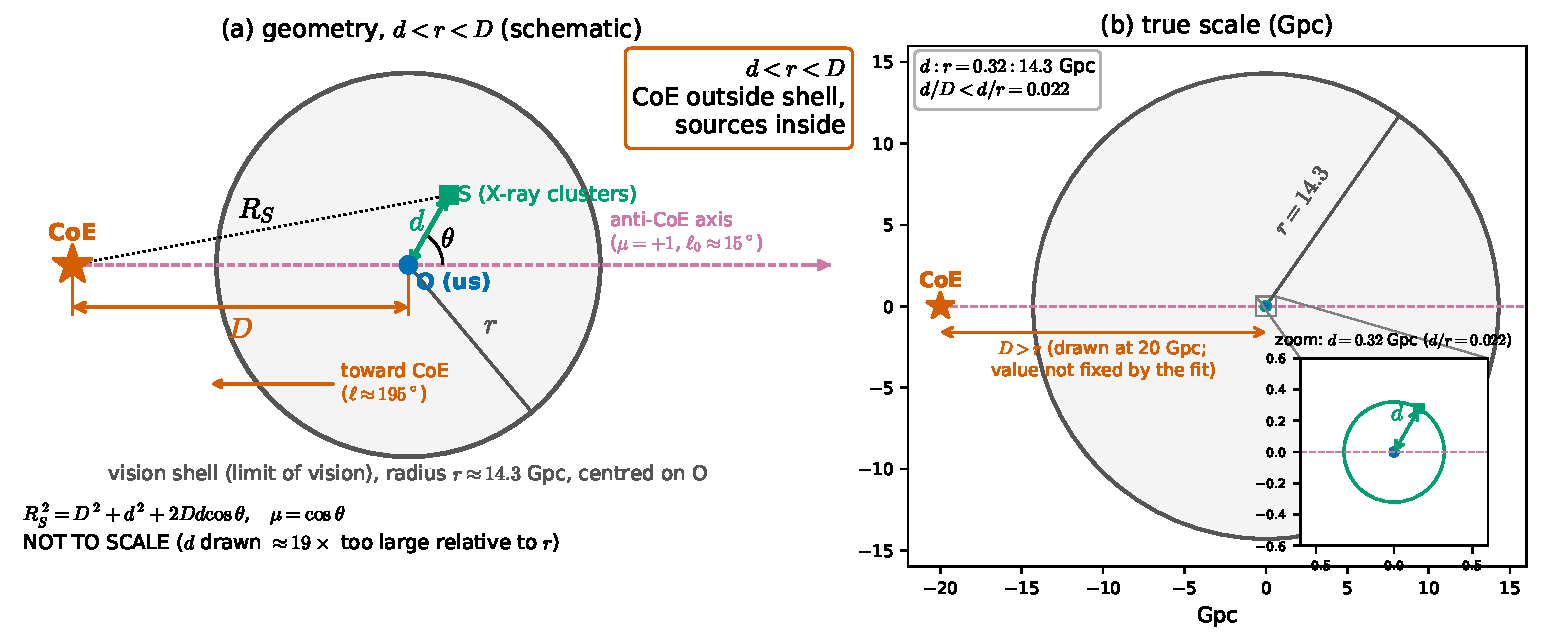
\includegraphics[width=\textwidth]{geometry_D_r_d.pdf}
\caption{Geometry for $d<r<D$. (a) Schematic, not to scale: CoE beyond the vision shell (radius $r$, centred on us), sources S inside at depth $d$, $R_S^2=D^2+d^2+2Dd\cos\theta$, $\theta$ from the anti-CoE axis. (b) True scale in Gpc: $d=0.32$ Gpc (green dot; zoom inset) against $r=14.3$ Gpc; $D>r$ is drawn at 20 Gpc for illustration only.}
\end{figure}

\paragraph{Caveats.}
(i) Full numerical model, re-optimized: $R^2=0.776\ (b_0=0^\circ),\ 0.777\ (15^\circ),\ 0.752\ (33.5^\circ)$, so $|b_0|=33.5^\circ$ is a truncation artifact and $b_0=0^\circ$--$15^\circ$ is not resolved.
At $b_0=0^\circ$: $\kappa\approx0.45$--$0.46$, $d/D\approx0.76$, $D/L\approx7.6$, $\ell_0\approx14.4^\circ$. At $b_0=15^\circ$: $\kappa\approx0.27$, $d/D\approx0.74$, $D/L\approx11.3$. All of these use $d/D\gg0.022$, so they violate $d<r<D$ as literal geometry.
(ii) $\kappa=GM(<D)/(H_0^2D^3)=M(<D)/[2M_{\rm crit}(<D)]$; $\rho_{\rm crit}=3H_0^2/8\pi G=1.36\times10^{11}M_\odot\,\mathrm{Mpc^{-3}}$ ($h=0.7$).
(iii) The coefficients $\tfrac92,\tfrac{15}{2}$ are point-mass values. (iv) The 71 sector points overlap and are not independent. (v) A single effective depth is used; the sample spans $z=0.003$--$0.45$, i.e.\ $d\lesssim1.9$ Gpc ($cz/H_0$), still $\ll r$.
\end{document}
